\documentclass{ximera}
\newcommand{\RR}{\mathbb R}
\renewcommand{\d}{\,d}
\newcommand{\dd}[2][]{\frac{d #1}{d #2}}
\renewcommand{\l}{\ell}
\newcommand{\ddx}{\frac{d}{dx}}
\newcommand{\dfn}{\textbf}
\newcommand{\eval}[1]{\bigg[ #1 \bigg]}

\author{Jim Talamo and Darry Andrews and Bart Snapp}

\begin{document}


Let $\vec{a} = \vector{-1,2}$ and $\vec{b}= \vector{1,2}$

\begin{problem}
  Give a calculator-ready expression for the angle between $\vec{a}$
  and $\vec{b}$.
  \begin{prompt}
    \[
    \theta = \answer{\arccos(3/5)}
    \]
  \end{prompt}

  \vfill
  
\end{problem}


\begin{problem}
  Compute: $\proj_{\vec{a}}(\vec{b})$
  \begin{prompt}
    \[
    \proj_{\vec{a}}(\vec{b}) = \vector{\answer{-3/5},\answer{6/5}}
    \]
  \end{prompt}

  \vfill
  
\end{problem}


\begin{problem}
  Sketch and label $\vec{a}$, $\vec{b}$, and $\proj_{\vec{a}}(\vec{b})$.
  \begin{image}
    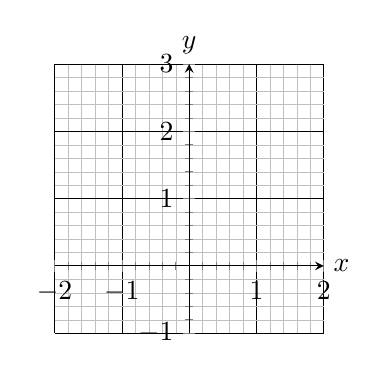
\begin{tikzpicture}
      \begin{axis}[
          xmin=-2,xmax=2,ymin=-1,ymax=3,
          clip=false,
          axis lines=center,
          width=5cm,
          height=5cm,
          xtick={-2,-1,...,2},
          ytick={-1,0,...,3},
          xlabel=$x$, ylabel=$y$,
          grid=both,
          grid style={line width=.1pt, draw=gray!50},major grid style={line width=.2pt,draw=black},
          minor tick num=4,
          every axis y label/.style={at=(current axis.above origin),anchor=south},
          every axis x label/.style={at=(current axis.right of origin),anchor=west},
        ]
        %\addplot[very thick,black,->] plot coordinates {(1,1) (4,2)};
        %\addplot[very thick,black,->] plot coordinates {(-1,0) (-3,3)};
        %\node[above] at (axis cs:2.5, 1.5) {$\vec{w}$};
        %\node[above] at (axis cs:-2, 1.5) {$\vec{v}$};
      \end{axis}
    \end{tikzpicture}
  \end{image}
  \begin{prompt}
      \begin{multipleChoice}
        \choice[correct]{I have drawn this.}
      \end{multipleChoice}
      \begin{feedback}
          \begin{image}
    \begin{tikzpicture}
      \begin{axis}[
          xmin=-2,xmax=2,ymin=-1,ymax=3,
          clip=false,
          axis lines=center,
          width=5cm,
          height=5cm,
          xtick={-2,-1,...,2},
          ytick={-1,0,...,3},
          xlabel=$x$, ylabel=$y$,
          grid=both,
          grid style={line width=.1pt, draw=gray!50},major grid style={line width=.2pt,draw=black},
          minor tick num=4,
          every axis y label/.style={at=(current axis.above origin),anchor=south},
          every axis x label/.style={at=(current axis.right of origin),anchor=west},
        ]
        \addplot[ultra thick,penColor,->] plot coordinates {(0,0) (1,2)};
        \addplot[ultra thick,red,->] plot coordinates {(0,0) (-1,2)};
        \addplot[thick,black,->] plot coordinates {(0,0) (-3/5,6/5)};
        \addplot[dashed] plot coordinates {(-3/5,6/5) (1,2)};
        \node[below right,penColor] at (axis cs:.5, 1) {$\vec{b}$};
        \node[below left,red] at (axis cs:-.75, 1.5
        ) {$\vec{a}$};
        \node[below left,black] at (axis cs:-.25,.7) {$\proj_{\vec{a}}(\vec{b})$};
      \end{axis}
    \end{tikzpicture}
  \end{image}
      \end{feedback}
  \end{prompt}

  \vfill
  
\end{problem}

\begin{problem}
  Find an orthogonal decomposition of $\vec{b}$ in terms of $\vec{a}$.
  \begin{prompt}
    \[
    \vec{b} = \underbrace{\vector{\answer{-3/5},\answer{6/5}}}_{\parallel \vec a} + \underbrace{\vector{ \answer{8/5},\answer{4/5}}}_{\perp\vec a}
    \]
  \end{prompt}

  \vfill
\end{problem}

\end{document}
